\documentclass[conference,compsoc]{IEEEtran}
\usepackage{ifpdf}
\usepackage[pdftex]{graphicx}
\usepackage[noadjust]{cite}
\usepackage{amsmath}
\usepackage[caption=false,font=footnotesize,labelfont=sf,textfont=sf]{subfig}
\usepackage{fixltx2e}
\hyphenation{op-tical net-works semi-conduc-tor}
\renewcommand{\citedash}{--}
\begin{document}

\title{Visual Dataflow Language for Small Robots Programming}

\author{
	\IEEEauthorblockN{Grogorii Zimin}
	\IEEEauthorblockA{
		Mathematics and Mechanics Faculty,\\
		SPbSU\\
		Saint-Petersburg, Russia \\
		Email: zimin.grigory@gmail.com
	}
	
	\and

	\IEEEauthorblockN{Dmitrii Mordvinov}
	\IEEEauthorblockA{
		Mathematics and Mechanics Faculty,\\
		SPbSU\\
		Saint-Petersburg, Russia \\
		Email: mordvinov.dmitry@gmail.com
	}
}

\maketitle



\begin{abstract}
REWRITE THIS SH..
The paper describes dataflow visual programming language based on DSM-approach. Its purpose is to be bridge between lightweight robotics languages for education and complex industrial languages. A short review of programming languages for robots is presented here. Also different approaches and architectures for developing control system for robots are considered. For demonstration of language usage, the paper provide solution for creating control system of robot based on subsumption architecture. 
\end{abstract}

\section{Introduction}

Programming languages for creating robotic controllers are actual topics of research oftenly discussed at major conferences, such as ICRA\cite{Icra} or IROS\cite{Iros2016}. Visual programming languages (VPLs) are also actively discussed for the last three decades, the largest conferences are held annually, e.g. VL/HCC\cite{VLHCC}. VPLs are oftenly applied in robotics domain\cite{banyasad2000visual,simpson2006mobile,simpson2008visual,posso2011process,diprose2011ruru} allowing to create and visualize robotic controllers. Robotic VPLs are commonly used for educational purposes, making possible for students of even junior schools to create robotic programs. There already exists a great number of educational robotic programming environments based on VPLs, e.g. NXT-G\cite{nxtg}, TRIK Studio\cite{trik}, ROBOLAB\cite{robolab}, also there are some academic tools implementing interesting and novel approaches to educational robotics programming\cite{banyasad2000visual,simpson2008visual,diprose2011ruru}.

Robotic control programs have reactive nature: they transform data which is continuously coming from multiple sensors into the impulses on actuators. For this reason dataflow languages (DFLs) are well-suitable for robotics programming. Many researchers denoted the conveniency of dataflow visual programming languages (DFVPLs)\cite{johnston2004advances}, finding them more useful than textual DFLs, for example, because data flows explicitly displayed on the diagram. There are large and complex general-purpose and domain-specific development environments such as LabVIEW\cite{labview} and Simulink\cite{simulink} that provide a large (and sometimes even cumbersome) set of libraries for robotics programming. More detailed discussion of robotics VPLs will be provided in section~\ref{sec:Overview}.

There is a large number of robotic constructor kits for learning the basics of robotics and cybernetics, such as LEGO MINDSTORMS\cite{legokit}, TRIK, ScratchDuino\cite{http://www.scratchduino.com/}. Modern programming languages that are used for programming those kits are based on the control flow model rather than on dataflow model. Control flow-based languages are good for solving scholar "toy" tasks, but may be inconvenient for programming more complex "real world" controllers that may be conveniently expresses on DFLs. The simple DFVPL may be considered as a useful step from educational VPLs to the programming languages that are used in unversities and industry. 


%Research-in-Progress Reports which should contain an abstract describing a problem of interest and particular goals of the research, a short description of related work with analysis of differences between the existing methods and the approach proposed by the author, a summary of results achieved and future work directions. The length of such papers should not exceed 6 pages.

In SPbSU cybernetic laboratory are conducted a number of studies aimed at improving the tools for design and programming of embedded systems for small robot platforms (e.g. LEGO, TRIK) using block diagrams\cite{}. Goal of research paper is the development of novel extensible tool for programming all small robot platforms which discussed above in dataflow style. While dataflow approach is commonly used approach when each element is executing in separate thread or process. Our approach avoids it, because it brings a large overhead on target platforms, details presented in section~\ref{sec:lang}.


The paper is organized as follows. An overview of robotics VPL and DFVPL is presented in section~\ref{sec:Overview}. A brief description of commonly used robots controller architectures is given in section~\ref{sec:architecture}. Then, description of our language are proposed in section~\ref{sec:lang}. Section~\ref{sec:robotControl} demonstrates typical robotic controller expressed in our language. Finally, the last section concludes the paper.



\section{Overview and background}
\label{sec:Overview}
Robot programming environment can be divided into three categories: educational, which allows you to program small robots; industrial, which have a rich toolkit for creating robots control systems and different models; academic, which implement new interesting ideas, however, are often not available for download, or are not robust.

To educational, for example, can be referred EV3 Software development environment for the Lego Mindstorms EV3 kit, IDE NXT-G and ROBOLAB for LEGO MINDSTORMS NXT kit, TRIK kit and IDE TRIK Studio. These IDE make it easy to solve typical robot control tasks, e.g., find a way out of the maze, drive along the line using sensors by creation a primitive control system, which purpose is to teach the users the basics of programming and robot control. But their simplicity is bound with poor flexibility of the language. Actually these IDEs provide a consistent model of the robot control based on control flow model, that is described by visual graphical models.

In the industry there are very popular general-purpose IDE LabVIEW from National Instruments with the DFVPL G, and programming environment Simulink developed by MathWorks for modeling different dynamic models or control systems. These software products offer to the users a huge range of models and libraries to create any control systems, test benches, real-time systems, using model-driven approach. In particular, LabVIEW provides opportunity programming small robots. Although there is known of LabVIEW usage for educational purposes\cite{1_gomez-de-gabriel_mandow_fernandez-lozano_garcia-cerezo_2011}, most of the time in the educational process is spent on the study of the medium itself, not algorithms and robotic approaches. It should be noted that these environments are distributed under the commercial license.

Another example of an industrial system is the Microsoft Robotics Developer Studio (MSRDS)\cite{jackson2007microsoft}, which is free for academic use, and allow to easy create distributed robotic systems in terms of data flow, which components are represented as web services. MSRDS officially supports multiple robotic platforms, e.g., LEGO NXT\cite{kim2007programming}, for which, however, It does not support offline mode. MSRDS has the ability to integrate with  custom robotic platforms, but this environment is not supported in 2014.
 
There are a lot of research in this area, e.g., dissertation\cite{banyasad2000visual} describes a visual programming language in terms of extended machines Moore, \cite{simpson2008visual},\cite{posso2011process} describe visual $occam\mbox{-}\pi$ program editor and tools $Transterpreter$, and its usage in  swarm robotics control system. Article\cite{diprose2011ruru} describes DFVPL for beginners and environment, which provides a comfortable interface. But the technology has too weak functionality and requires significant improvements, and doesn't available for download.

Based on the overview it is clear that no one of these environments is not suitable for programming TRIK in terms of data flows. At the same time closest to the desirable is TRIK Studio, as it is the only medium, which distributed with open source with a highly scalable architecture, that has the ability to extend itself by new VPL for robots and provides opportunity to reuse code base of "routine" operations such as the interaction with the robot.


\section{Robots control architectures}
\label{sec:architecture}
%С выходом статьи Родни Брукса\cite{1_brooks_1986}, описывающей возможность декомпозировать задачу управления роботом горизонтально на уровни ответственности, стало возможно проще и эффективнее решать "составные" задачи управления, как, например, задачи телеоператорского контроля балансирующего робота с автоматическим избеганием столкновений с препятствиями. Языки потоков данных удачно подходят под эту модель, что подтверждают неоднократные публикации на эту тему: \cite{simpson2006mobile}, \cite{banyasad2000visual}, \cite{posso2011process}, \cite{proetzsch2007behaviour}. В этой модели, система управления представлена как набор уровней ответственности, которые отвечают за различные модели поведения робота и строятся последовательно. При этом, по очевидным причинам, упрощается масштабируемость системы и увеличивается ее отказоустойчивость.

%	У архитектуры Брукса есть множество альтернатив, к примеру, <<Колония>> Джонотана Коннеля, архитектура <<выбора-действия>> Патти Мэйса, <<схема двигателя>> Рональда Аркина\cite{simpson2009toward}, модель управления для системы Телеробота\cite{albus1989nasa}. Однако среди упомянутых подходов, подход Брукса является наиболее популярным, поэтому основопологающей концепцией разрабатывамого языка было решено сделать поддержку именно его.


\section{Description of language}
\label{sec:lang}
%Развитие модельно-ориентированного (\textit{DSM}) подхода\cite{koznov2008} позволило быстро создавать достаточно сложные визуальные языки программирования. Среда программирования TRIK Studio является примером системы, созданной с применением DSM-подхода на базе платформы QReal\cite{qrealMeta}\cite{kuzenkova2013qreal}. Основываясь на промышленном опыте разработчиков TRIK Studio, было решено создавать потоковый язык программирования роботов на базе платформы QReal. Первый прототип языка был создан в течение недели. На момент написания статьи язык и средства его поддержки находятся в активной разработке. Опишем некоторые особенности разрабатываемой технологии.

%\begin{itemize}
%\item Архитектура Брукса легко выражается средствами языка.
%\item Диаграммы поведения роботов, так же как и в TRIK Studio, имеют возможность быть проинтерпретированными на двумерной имитационной модели робота. 
%\item В ближайших планах стоит генерация диаграмм потоков данных в текстовые языки, используемые для программирования TRIK --- в первую очередь, JavaScript, F\#\cite{kirsanov2014robotics} и Kotlin.
%\end{itemize}

%\section*{Элементы языка}
%Элементы языка можно разделить по назначению на несколько групп.

%\begin{itemize}
%\item \textit{Элемент потока данных}. Связь, реализующая поток для передачи данных. 
%\item \textit{Блоки управления приводами}. Блоки принимающие числовые значения, отвечающие за подачу импульсов на приводы (силовые моторы, сервомоторы и т.д.).
%\item \textit{Блоки считывания данных с сенсоров}. Блоки, генерирующие соответствующие значения, которые подлежат дальнейшей обработке.
%\item \textit{Блоки синхронизации и фильтрации}. Позволяют временно блокировать передачу данных, устанавливать количество наборов пропускаемых данных и время между отправками. 
%\item \textit{Блоки поддержки устройств ввода}. Считывают данные с устройств операторского контроля (в данный момент поддержан только джойстик, в планах --- компьютерная мышь и клавиатура). 
%\item \textit{Блоки рисования на экране}. Отвечают за векторное и растровое рисование на экране.
%\item \textit{Блоки видеозрения}. Предоставляют доступ ко всем возможностям видеозрения контроллера TRIK.
%\item \textit{Блоки взаимодействия между роботами}. Отвечают за групповую координацию роботов.
%\item \textit{Блок текстового программирования}. Блок, позволяющий произвести обработку входных данных на текстовом языке (статически типизируемом диалекте Lua, поддержка которого <<унаследована>> от кодовой базы TRIK Studio). Чаще всего такой блок будет использоваться для задания математических операций над данными.
%\item \textit{Блоки управляющих конструкций}. Включают циклы, условные развилки, множественный выбор, распараллеливание, подавление и ингибицию, блок <<Подпрограмма>> для переиспользования кода. Последние четыре блока обеспечивают поддержку архитектуры Брукса в языке.

%\end{itemize} 

\section{Robot control system}
\label{sec:robotControl}

%Рассмотрим задачу управления движением робота при помощи джойстика, при условии, что робот сам избегает лобовых столкновений с припятствиями. Предполагается, что программа пишется для двухколесного мобильного робота, оборудованного спереди инфракрасными датчиками расстояния, для управления колесами используются силовые моторы.

%Разобьем задачу на два уровня поведения. Первый будет отвечать за обслуживание запросов пользователя. Второй будет ответственен за избегание столкновений: если робот близок к столкновению, то он должен уклониться от препятствия вне зависимости от того, что нажимает пользователь на пульте. 

%Рассмотрим первый уровень (рис.~\ref{image:layer1}). Пользователь управляет роботом посредством джойстика. Джойстик генерирует данные, соответствующие нажатиям кнопок или манипулирований рычагом направления. Для простоты считаем, что нажатие любой кнопки завершит программу управления роботом. Данные с рычага преобразуются блоком текстового программирования в соответствующие импульсы моторов робота, которые в данном случае передаются <<заглушкам>>, которые связаны с выходными портами блока <<Подпрограмма>>. 
%\begin{figure}[ht]
%	\centering
%	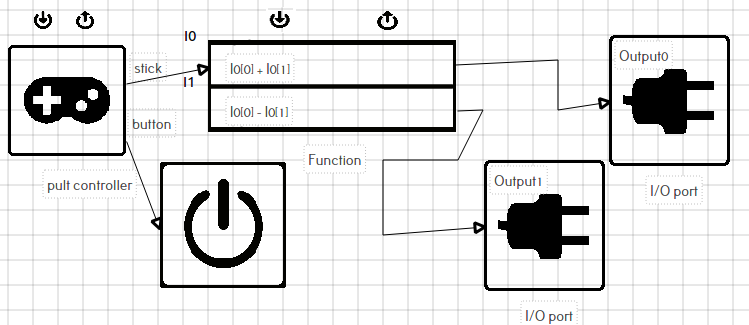
\includegraphics[width=3.5in]{pultLayer.png}
%	\caption{Уровень управления с пульта.}
%	\label{image:layer1}
%\end{figure}

%Рассмотрим второй уровень (рис.~\ref{image:layer2}): данные с датчиков расстояния собираются в вектор и передаются фильтру, который при опасности столкновения отправляет данные дальше в блок математической обработки (если условие не выполнилось, управление может быть передано по потоку <<ошибки>>, в данной программе этот поток не указан; также между проверками условия приходящие данные не обрабатываются (теряются) в течение установленного пользователем времени). В блоке математической обработки вычисляется мощность, которую необходимо подать на 2 мотора. Вычисленные значения передаются выходным портам.
%\begin{figure}[ht]
%	\centering
%	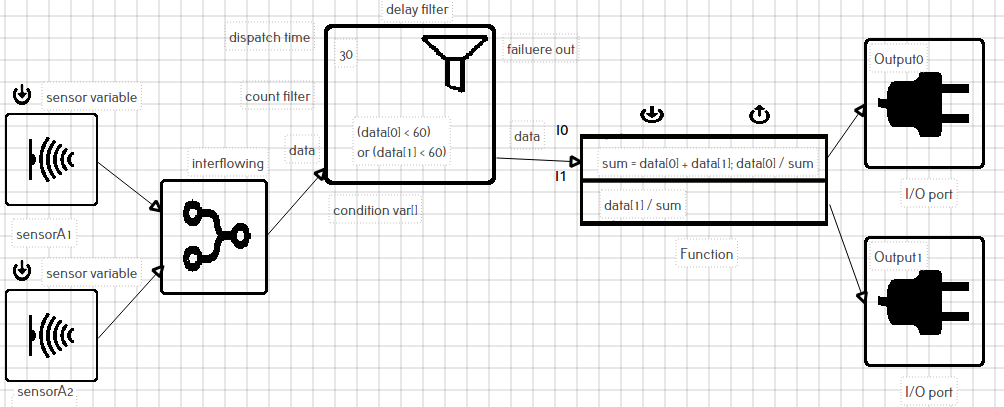
\includegraphics[width=3.5in]{collisionLayer.png}
%	\caption{Уровень избегания столкновений.}
%	\label{image:layer2}
%\end{figure}

%\begin{figure}[ht]
%	\centering
%	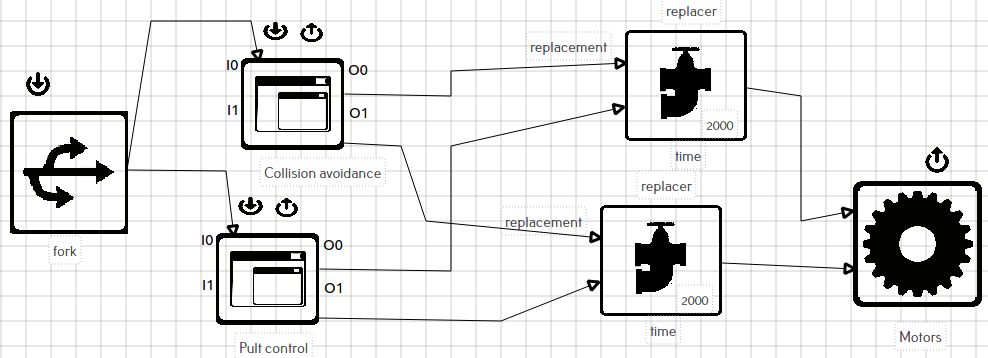
\includegraphics[width=3.5in]{programScreen.png}
%	\caption{Программа управления роботом.}
%	\label{image:prog}
%\end{figure}

%Имея два поведения, создаем управление роботом в модели Брукса (рис.~\ref{image:prog}). С помощью блока распараллеливания запускаем уровни поведения. Каждый уровень генерирует данные, соответствующие мощностям моторов, передаваемые на блок управления силовыми моторами. Так как второй уровень ответственности должен не позволить столкнуться с препятствием, его значения подавляют значения, полученные с первого уровня, с помощью блоков <<Подавления>>.

\section{Future works}
\label{sec:Future}

\section{Conclusion}
%На момент написания статьи был реализован прототип технологии програмирования роботов TRIK в терминах потоков данных. Система предоставляет возможность интерпретации диаграмм на двумерной имитационной модели робота и (в ближайшем будущем) генерации кода из диаграмм в текстовые языки, используемые для программирования TRIK (JavaScript, F\# и Kotlin). Также технология предоставляет поддержку архитектуры Брукса на уровне языка, что продемонстрировано в статье на примере операторского управления роботом с автоматическим избеганием столковений.

%Полученная система может рассматриваться как платформа для дальнейших научных исследований. К примеру, интересной представляется автоматическая генерации метамодели языка по спецификациям ПО промежуточного уровня на роботе (к примеру, ROS\footnote{http://www.ros.org/ [Дата обращения: 10 марта 2016]}). Другим направлением возможной работы является описание строгой семантики языка для применения различных формальных методов анализа программ, выраженных в нем.

\newpage
\bibliography{IEEEbibl}
\bibliographystyle{IEEEtran}
\end{document}
